% Name: Cellular automaton
% Description: Rule 30: the new state of a cell for each of the eight neighborhoods, and the first eight rows grown from a single live cell.
% Tags: cellular automaton, Rule 30, Wolfram, elementary automaton

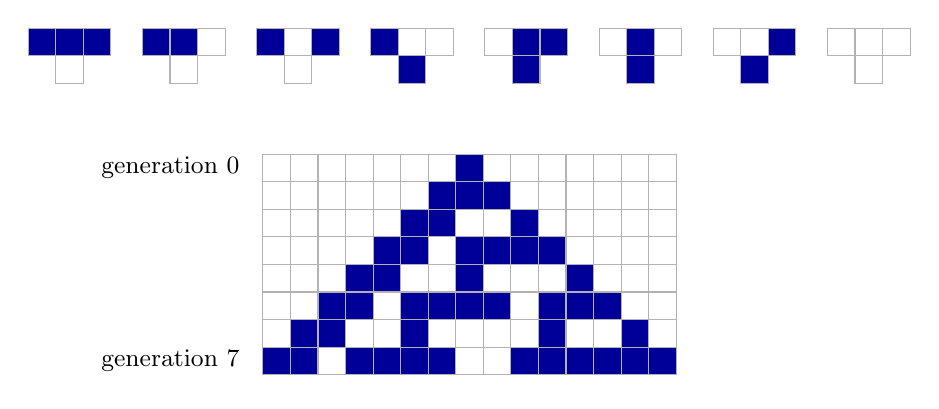
\begin{tikzpicture}[cell/.style={draw=gray!60, minimum size=3.5mm, inner sep=0pt}, live/.style={cell, fill=blue!60!black}, s0/.style={cell}, s1/.style={live}]
  % The rule: neighborhoods 111 down to 000 map to the bits of 30 = 00011110.
  \foreach \l/\c/\r/\out [count=\i from 0] in {1/1/1/0, 1/1/0/0, 1/0/1/0, 1/0/0/1, 0/1/1/1, 0/1/0/1, 0/0/1/1, 0/0/0/0} {
    \foreach \v [count=\j from 0] in {\l, \c, \r}
      \node[s\v] at (1.45*\i+0.35*\j-5.43,1.6) {};
    \node[s\out] at (1.45*\i-5.08,1.25) {};
  }
  % Generations 0 to 7, as computed from the rule; each list gives the live cells' offsets from the center.
  \foreach \row [count=\g from 0] in {{0}, {-1,0,1}, {-2,-1,2}, {-3,-2,0,1,2,3}, {-4,-3,0,4}, {-5,-4,-2,-1,0,1,3,4,5}, {-6,-5,-2,3,6}, {-7,-6,-4,-3,-2,-1,2,3,4,5,6,7}} {
    \foreach \x in {-7,...,7} \node[cell] at (0.35*\x,-0.35*\g) {};
    \foreach \x in \row \node[live] at (0.35*\x,-0.35*\g) {};
  }
  \node[font=\small, anchor=east] at (-2.8,0) {generation 0};
  \node[font=\small, anchor=east] at (-2.8,-2.45) {generation 7};
\end{tikzpicture}
